\documentclass[twocolumn]{article}

\usepackage{graphicx}
\renewcommand{\partname}{}

\begin{document}	
	\twocolumn[
	\begin{@twocolumnfalse}
		\author{Michael Sedrak \\ m.sedrak@live.com}
		\title{Solving TSP With Genetic Algorithms}
		\maketitle
		\begin{abstract}
			Lorem ipsum dolor sit amet, consectetur adipiscing elit. Suspendisse condimentum, urna nec luctus tincidunt, nisi augue vehicula nulla, sit amet sollicitudin nisi nibh eget diam. Vivamus maximus tortor dolor, non porttitor urna vestibulum eu. Nullam maximus in massa eu lacinia. Curabitur ac risus ac elit euismod placerat quis eu odio. Sed ante ex, congue sit amet enim et, aliquam egestas turpis. Cras purus ex, viverra sit amet augue id, tempus ultricies risus. Aenean eget vestibulum orci. Ut enim nisi, tempor id urna et, dignissim ornare lectus. Nunc lobortis risus neque, a fermentum ante consequat ac. Fusce mollis pretium pellentesque. Vestibulum fermentum ornare elementum. Nam rutrum sem ut est mollis consequat. Morbi at faucibus mi. In ultricies justo non lorem varius, non tristique ante suscipit. Curabitur eget diam tincidunt, venenatis enim sagittis, malesuada magna. Nullam in urna a odio finibus tristique.
		\end{abstract}
	\end{@twocolumnfalse}
	]
	
	%% Document body starts from here
	\part{Methodology}
	\section{Dataset}
	Datasets for TSP problem contain a wide variety of formats. Cities across a country, VLSI nodes or travelling across the Mona Lisa drawing. But they are all similar in the aspect of the data structure. The structure is a 2-D coordinate point system with euclidean distances as the distance between nodes.
	For our work we selected the Uruguay dataset from the national dataset collection. Uruguay dataset is characterised by 
	\begin{itemize}
	\item 734 unique points (no duplicates)
	\item Optimal tour of length 79114
	\end{itemize}
	\begin{figure}[h!]
	\centering
		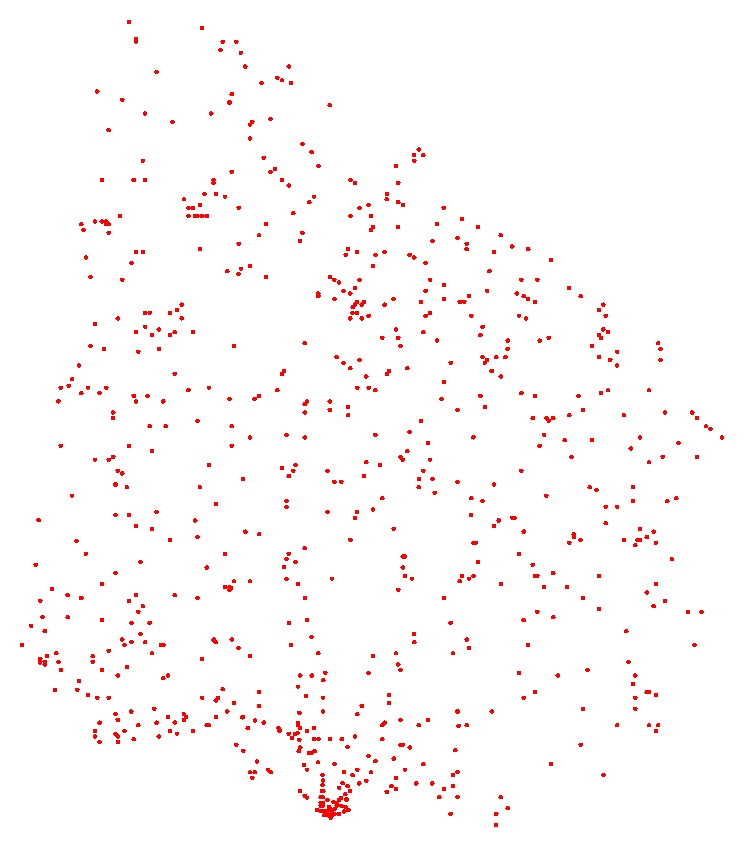
\includegraphics[scale=0.3]{./tex/uypoints.jpg}
	\caption{XY coordinate representation of Uruguay dataset}
	\label{fig:uruguay}
	\end{figure}
	A graphical representation of the coordinates of the dataset is shown in figure \ref{fig:uruguay}
\end{document}
